% ----------------------------------------------------------------------
%                   LATEX TEMPLATE FOR PhD THESIS
% ----------------------------------------------------------------------

% based on Harish Bhanderi's PhD/MPhil template, then Uni Cambridge
% http://www-h.eng.cam.ac.uk/help/tpl/textprocessing/ThesisStyle/
% corrected and extended in 2007 by Jakob Suckale, then MPI-CBG PhD programme
% and made available through OpenWetWare.org - the free biology wiki
% Modified to conform with University of Pennsylvania Thesis Requirements 
% by Alan Meert & David F. Moore, 2013, Dept. of Physics and Astronomy

%: --------------------------------------------------------------------------
%: Style file for Latex
%: Specify openright if printing double-sided, openany if single-sided
%: --------------------------------------------------------------------------
\documentclass[11pt, openany, oneside]{Latex/Classes/PhDthesisPSnPDF}
\usepackage{lipsum} % this just creates filler text when needed

%: --------------------------------------------------------------------------
%: Use Natbib for non-standard citations 
%: --------------------------------------------------------------------------
%: uncomment below to change from standard TeX in-text citations to
%: author-year in-text citations. Should be used together with the 
%: PhDbiblio-intext-twoauth.bst file (included with this project) or 
%: some other acceptable .bst file 
%: --------------------------------------------------------------------------

%\usepackage[authoryear]{natbib}
%  \bibpunct{(}{)}{;}{a}{}{,}

%: --------------------------------------------------------------------------
%: The end user may modify these files to personalize and define macros
%: --------------------------------------------------------------------------
\usepackage{Latex/StyleFiles/UserDefs} % Define any user-defined Macros and functions in this file.
% This file contains macros that can be called up from connected TeX files
% It helps to summarise repeated code, e.g. figure insertion (see below).

% insert a centered figure with caption and description
% parameters 1:filename, 2:title, 3:description and label
\newcommand{\figuremacro}[3]{
	\begin{figure}[htbp]
		\centering
		\includegraphics[width=1\textwidth]{#1}
		\caption[#2]{\textbf{#2} - #3}
		\label{#1}
	\end{figure}
}

% insert a centered figure with caption and description AND WIDTH
% parameters 1:filename, 2:title, 3:description and label, 4: textwidth
% textwidth 1 means as text, 0.5 means half the width of the text
\newcommand{\figuremacroW}[4]{
	\begin{figure}[htbp]
		\centering
		\includegraphics[width=#4\textwidth]{#1}
		\caption[#2]{\textbf{#2} - #3}
		\label{#1}
	\end{figure}
}

% inserts a figure with wrapped around text; only suitable for NARROW figs
% o is for outside on a double paged document; others: l, r, i(inside)
% text and figure will each be half of the document width
% note: long captions often crash with adjacent content; take care
% in general: above 2 macro produce more reliable layout
\newcommand{\figuremacroN}[3]{
	\begin{wrapfigure}{o}{0.5\textwidth}
		\centering
		\includegraphics[width=0.48\textwidth]{#1}
		\caption[#2]{{\small\textbf{#2} - #3}}
		\label{#1}
	\end{wrapfigure}
}

% predefined commands by Harish
\newcommand{\PdfPsText}[2]{
  \ifpdf
     #1
  \else
     #2
  \fi
}

\newcommand{\IncludeGraphicsH}[3]{
  \PdfPsText{\includegraphics[height=#2]{#1}}{\includegraphics[bb = #3, height=#2]{#1}}
}

\newcommand{\IncludeGraphicsW}[3]{
  \PdfPsText{\includegraphics[width=#2]{#1}}{\includegraphics[bb = #3, width=#2]{#1}}
}

\newcommand{\InsertFig}[3]{
  \begin{figure}[!htbp]
    \begin{center}
      \leavevmode
      #1
      \caption{#2}
      \label{#3}
    \end{center}
  \end{figure}
}


%%% Local Variables: 
%%% mode: latex
%%% TeX-master: "~/Documents/LaTeX/CUEDThesisPSnPDF/thesis"
%%% End: 
 % Some prewritten Macros for Use in Latex

\usepackage[T3]{fontenc}
\usepackage{charter}
\usepackage[expert]{mathdesign}

%: ----------------------------------------------------------------------
%:                  User information
% -----------------------------------------------------------------------

% DISSERTATION TITLE
\title{Mapping Functional Architecture in Neocortical Epileptic Networks} %The title of your thesis
% Optional Sub-title
%\SubTitle{Mapping Epileptic Networks} %comment if you don't want a subtitle

%YOU 
\author{Ankit Narendra Khambhati}

% Degree information
\DegreeDate{2015} % expected year of graduation.
\degree{Doctor of Philosophy}

%YOUR DEPARTMENT and UNIVERSITY
\collegeordept{Bioengineering}
\university{University of Pennsylvania}

%YOUR ADVISOR
\supervisor[Professor of Neurology \& Bioengineering]{Brian Litt}

% Your Department Graduate chair
\gradchair[Professor of Bioengineering]{Jason Burdick}

% Additional Commitee Members [title]{Name}
\firstcomittee[Professor of Electrical and Systems Engineering \& Computer and Information Science]{Daniel D. Lee}
\secondcomittee[Skirkanich Assistant Professor of Innovation of Bioengineering]{Danielle S. Bassett}
\thirdcomittee[Assistant Professor of Neurosurgery, Perelman School of Engineering]{Timothy H. Lucas}


% Copyright statement of your choice
\CopyrightStatement{This work is licensed under the Creative Commons
Attribution-NonCommercial-ShareAlike 4.0 License.\newline
\noindent To view a copy of this license, visit
\href{http://creativecommons.org/licenses/by-nc-sa/4.0/}{%
http://creativecommons.org/licenses/by-nc-sa/4.0/}
}

%: --------------------------------------------------------------
%:                  BEGIN THE DOCUMENT!!!
% --------------------------------------------------------------
\begin{document}

% sets line spacing
\renewcommand\baselinestretch{1.2}
\baselineskip=18pt plus1pt

%: ------------------------------------------------------------------------
%:                  FRONT MATTER: dedications, abstract,..
% -------------------------------------------------------------------------

%: ----------------------- generate cover page ----------------------------
\maketitle  

%: ----------------------- generate copyright page ------------------------
\makecopyright  

%: ----------------------- Include a Dedication ---------------------------
% Thesis Dedictation ---------------------------------------------------

\begin{dedication} %this creates the heading for the dedication page

\large\emph{To Baa, \\ \indent for her strength, \\ and Dada, \\ \indent for his resolve.}

\end{dedication}

% ----------------------------------------------------------------------


%: ----------------------- Include an Acknowledgement ---------------------
% Thesis Acknowledgements ------------------------------------------------

\begin{acknowledgements}
Five years ago, the opportunity to conduct meaningful and clinically impactful brain research seemed a far off pipe dream. First and foremost, I thank my advisor and mentor, Brian Litt, for placing his trust in me and inviting me to pursue Master's and Doctoral-level research. Brian, I am indebted to you for showing me how to ask big-picture questions and instilling in me the grander vision of conducting research to help patients in the near-term. You encouraged my intellectual curiosity and afforded me the freedom to explore new domains of scientific work -- in hopes that we would understand just a little bit more about epilepsy and its complexity. You also provided me an important glimpse of academic life as a teacher and showed me how to advise younger students on harnessing their skills and pursuing meaningful careers. As a team player who humbly distributes credit in times of success, you have imprinted on me a passion for collaborative research and integrating knowledge across discplines.

Brian also deserves credit for introducing me to my second mentor, Danielle Bassett, who has played an instrumental role guiding the technical aspects of my work. Dani, your willingness and enthusiasm to discuss theory, absurd hypotheses, research papers, and academic life is a model for the type of academician I can only dream of becoming. Most importantly, you've taught me that being an excellent researcher requires more than good technical skill and vision -- it requires artistry in effective communication and language.

I would also like to extend gratitude to Timothy Lucas, for providing added perspective outside of the computational lab, in the operating room. As a neurosurgeon, you opened my eyes to a second world of clinical challenges associated with translational research, especially in epilepsy. I appreciate your patience with our Neuralynx team and thank you for valuable clinical and technical insights to overcome critical hurdles.

I would be remiss not to mention Gershon Buchsbaum as an invaluable mentor early in my dissertation work. You helped me navigate the program goals and milestones, and encouraged me to ask questions, to be thorough, and to verify hypotheses. I owe much of my thesis focus in examining spatial distributions of epileptic activity to our early discussions.

I must also thank the clinicians -- Kate Davis, Shawniqua Williams, Stephanie Chen, Brian Oommen, and Mesha-Gay Brown -- who have provided helpful discussion and devoted extended time to marking seizures in the 22 patient data set analyzed in this thesis.

Furthermore, I thank Tyler Blevins for all his time and effort in organizing and automating the analysis of these large data sets on the IEEG Portal. To say the least, without the continuous effort by Jacqueline Boccanfuso, John Frommeyer and Joost Wagenaar in actively maintaining the IEEG infrastructure, the valuable patient data for this thesis might still be sitting in archived hospital servers.

Carolyn Wilkinson, Ruth Krieger, Jacqueline Boccanfuso, and Ashley Brito deserve many thanks in their many hats as data coordinators, proofreaders, event planners and all-in-all making the lab run as smooth as butter.

I especially thank Hank Bink, Lohith Kini, and Hoameng Ung, who have become close friends. Hank, the tall guy sitting directly to my left, has been my source of comic relief and my teacher of pop culture over the last five years. I also thank my close friends outside of lab for helping me maintain a healthy work-life balance.

Mom, Dad, and Kaushal -- your life-long support and love is the only reason I have made it to where I am. You have all stuck behind me, even through my most stubborn times, and no words can express the amount of gratitude I feel. Finally, Kinjal, you balance my insanity with your sanity and poise. Even on the grimmest days of my PhD, you managed to keep me going with all smiles. If the past few years are any indication, this is just the start of a great adventure with you.

\end{acknowledgements}

% ------------------------------------------------------------------------




%: ----------------------- abstract ---------------------------------------
% Thesis Abstract -----------------------------------------------------

\begin{abstracts}
Epilepsy is a debilitating brain disorder that causes recurring seizures in approximately 60 million people worldwide. For the one-third of epilepsy patients whose seizures are refractory to medication, effective therapy relies on reliably mapping the epileptic network through neural sensors recording the electrocorticogram to determine the seizure origin as a target for surgical resection, or more recently implantable devices. Mapping functional architecture in the epileptic network is promising for objectively localizing cortical targets for therapy in cases of neocortical refractory epilepsy, where post-surgical seizure freedom is unfavorable when cortical structures responsible for generating seizures are difficult to delineate. In this work, we develop and apply network models for analyzing and interrogating the role of fine-grain functional architecture during epileptic events in human neocortical networks. We first develop and validate a model for objectively identifying regions of the epileptic network that drive seizure dynamics. We then develop and validate a model for mapping latent structure in the epileptic network, predicting regions driving seizure generation from functional architecture during ``normal'', baseline brain states. Lastly, we devise and apply a novel platform for predicting network response to targeted lesioning of neocortical structures, revealing key control areas that influence the spread of seizures to broader network regions. The outcomes of this work demonstrate network models can objectively identify and predict targets for treating neocortical epilepsy, blueprint potential control strategies to limit seizure spread, and are poised for clinical translation in the near future.
\end{abstracts}

% ---------------------------------------------------------------------- 


%: ----------------------- generate Table of Contents ---------------------
\setcounter{secnumdepth}{3} % organisational level that receives a numbers
\setcounter{tocdepth}{3}    % print table of contents for level 3
\tableofcontents            % print the table of contents
% levels are: 0 - chapter, 1 - section, 2 - subsection, 3 - subsection


%: ----------------------- generate list of tables ------------------------
\listoftables  % print list of tables

%: ----------------------- generate list of figures ------------------------
\listoffigures	

%: ----------------------- Preface -----------------------------------------
% Thesis Preface -----------------------------------------------------

\begin{preface}

Perhaps you feel inclined to preface your work with poetic 
self-reflection about why you took up this project? Maybe a story 
that's kind of boring and ends with a joke that's not funny? Go for it!


\end{preface}

% ---------------------------------------------------------------------- 



%: -------------------------------------------------------------------------
%:                  MAIN DOCUMENT SECTION
% --------------------------------------------------------------------------

\mainmatter


%: ----------------------- introduction file header -----------------------
\chapter{Introduction}

% the code below specifies where the figures are stored
\ifpdf
    \graphicspath{{introduction/figures/PNG/}{introduction/figures/PDF/}{introduction/figures/}}
\else
    \graphicspath{{introduction/figures/EPS/}{introduction/figures/}}
\fi

% ----------------------------------------------------------------------
%: ----------------------- introduction content ----------------------- 
% ----------------------------------------------------------------------

\section{put section name here} 
Any organised system requires energy, be it a machine of some kind or a live organism. Energy is needed to win the uphill battle against entropy and pull together lifeless molecules to be able to do something in this world, like complete a PhD\nomenclature[Zp]{Ph.D}{Acronym}.

\subsection{Name your subsection}
The machines that enable us to do science like sizzling electricity but at a controlled voltage\index{voltage}. Earth's living beings are no different, except that they have developed another preference. They thrive on various chemicals \citep{name06}. \lipsum


% ----------------------------------------------------------------------



	

\chapter{Background}
\label{ch:background}

% the code below specifies where the figures are stored
\ifpdf
    \graphicspath{{chapters/ch2_figures/PNG/}{chapters/ch2_figures/PDF/}{chapters/ch2_figures/}}
\else
    \graphicspath{{chapters/ch2_figures/EPS/}{chapters/ch2_figures/}}
\fi


% ----------------------------------------------------------------------
%: ----------------------- content ----------------------- 
% ----------------------------------------------------------------------

\section{Diagnosis and Treatment of Neocortical Epilepsy}
In this dissertation we focus on a population of drug-resistant epilepsy patients whose seizures arise in the neocortex, or the superficial tissue comprising the first functional layers of gray-matter in the brain (\textbf{Fig.~\ref{epilepsy_type}}). Neocortical epilepsy cases are among the most difficult epilepsy types to treat, because their etiology and localization is unique to each patient. Neocortical epilepsy has a variety of causes ranging from genetic to structural and metabolic, and in some cases the cause cannot be identified \cite{berg2010revised}. Of those patients with neocortical epilepsy, seizures may focally originate in the frontal lobe, temporal lobe, occipital lobe, parietal lobe, or from a combination of these regions.

\begin{figure}
\centering
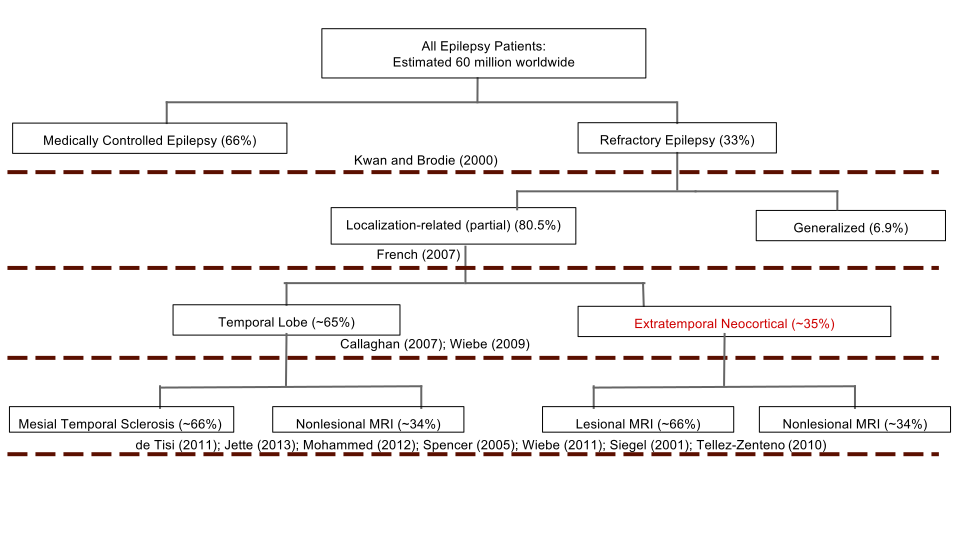
\includegraphics[width=\textwidth]{epilepsy_type}
\caption[Chart of epilepsy types]{\textbf{Population distribution of epilepsy types.} The distribution of patients with different types of epilepsies. The literature sources used to estimate population percentage is listed at each level. The focus of this work is extratemporal neocortical epilepsy, which has a prevalence of $\approx$6 million people.}
\label{epilepsy_type}
\end{figure}

\subsection{Clinical Imaging to Localize Structural and Functional Abnormalities}
While intracranial monitoring of neural activity associated with epileptic events is indispensable for identifying the seizure origin, multi-modal imaging can often identify lesions (\textbf{Fig.~\ref{typeIIfcd}}) (e.g. focal cortical dysplasia, tuberous sclerosis, other malformations of cortical development), which when resected lead to significantly better odds (2.9 times) of seizure freedom than in cases where imaging returns negative findings \cite{tellez-zenteno2010surgical}. For cases with unknown etiology, only $\approx$54\% of patients attain favorable seizure freedom (Engel score I or II) \cite{lee2005surgical}. Even in cases where no clear lesions are evident on MRI, clinicians collect a variety of imaging modalities providing orthogonal information about the epileptic network. We briefly introduce some of these imaging techniques below \cite{kuzniecky2002neuroimaging}:

\begin{figure}
\centering
\includegraphics[width=0.25\textwidth]{typeIIfcd_mri}
\caption[Example of brain lesion]{\textbf{Example of epileptogenic brain lesion.} A T2-weighted coronal FLAIR image displaying hyperintensity (white) in the inferior precuneus corresponding to a Type IIB focal cortical dysplasia, a common lesion underlying the development of focal seizures \cite{gaillard2015focal}.}
\label{typeIIfcd}
\end{figure}

\paragraph{Magnetic Resonance Imaging (MRI)}
T1 or T2-weighted imaging sequence that enables delineation of gray- and white-matter brain tissue. This imaging modality is most widely used for localizing aberrant migration of neural tissue associated with developmental disorders and investigating anatomical changes due to brain injury. Epilepsy cases with unremarkable MRI are colloquially considered \textit{non-lesional}.

\paragraph{Single Photon Emission Computed Tomography (SPECT)}
SPECT imaging is used in conjunction with an injectable radioactive tracer, which together yield a dynamic or static picture of blood perfusion through the brain. SPECT may be conducted during the ictal period to identify patterns of seizure onset and spread and, when compared to baseline interictal SPECT, can localize portions of the epileptic network in 70--90\% of patients \cite{kuzniecky2002neuroimaging}. The challenge for clinicians is accurate timing of conducting a SPECT study during seizures, which occur infrequently.

\paragraph{Positron Emission Tomography (PET)}
For epilepsy patients, PET is often used in conjunction with the radioactive tracer fluorodeoxyglucose (FDG), which together yield an estimate of metabolic activity in imaged tissue. While interictal PET has shown utility in localizing abnormalities in temporal lobe epilepsy, results are less promising for neocortical epilepsy. 

\subsection{Intracranial Monitoring of Brain Electrophysiology}
Although structural and functional imaging modalities provide significant information regarding abnormal brain tissue, the electrophysiology of neural circuits provide the clearest evidence of dysfunction when diagnosing epilepsy. A patient's neurological team will compile results from imaging and phase-I monitoring of scalp electroencephalography (EEG) and plan an invasive surgery to implant sub-dural, intracranial sensors for monitoring the electrocorticogram (ECoG) (\textbf{Fig.~\ref{intracranial_electrodes}}).  

\begin{figure}
\centering
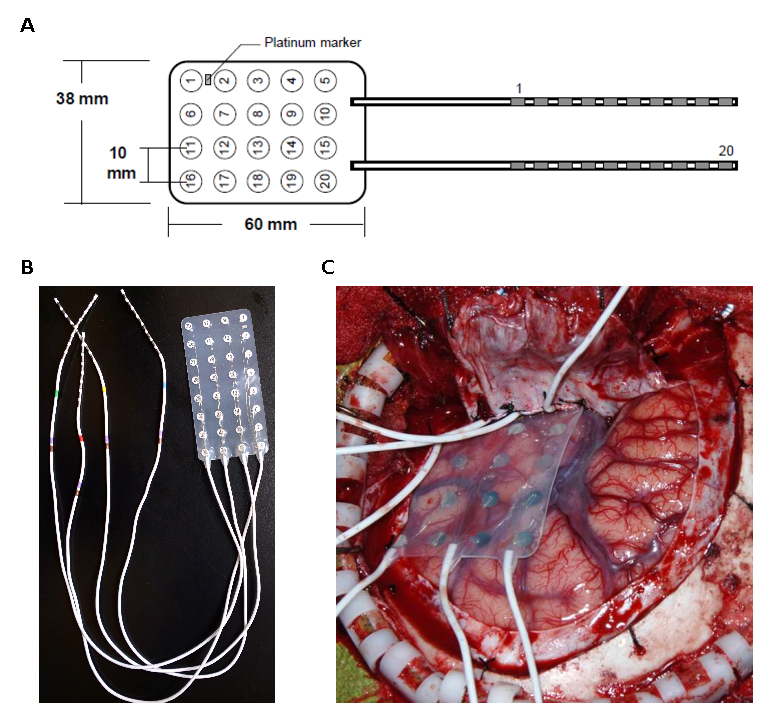
\includegraphics[width=\textwidth]{intracranial_electrodes}
\caption[Implantation of intracranial electrodes]{\textbf{Intracranial electrodes for monitoring epileptic cortex.} (\textbf{A}) Schematic of clinical-scale intracranial electrode with 20 sensors arranged in 4x5 configuration. Center-to-center distance between sensors is 10mm, and each sensor as a diameter of 4mm with 2.3mm exposed to the sub-dural cortical surface. (\textbf{B}) Photograph of a similar electrode with 32 sensors in 4x8 configuration. (\textbf{C}) Intraoperative photograph of implanted electrode in human epilepsy patient with reference to gyral, sulcal, and vascular anatomy.}
\label{intracranial_electrodes}
\end{figure}

Each sensor of an ECoG electrode is made from platinum-iridium and captures the local field potential (LFP) of neural activity from superficial layers of the neocortex \cite{buzsaki2012origin}. This LFP represents the extracellular voltage deflection from an aggregated population of neurons and is comprised of the population's synaptic activity and action potential firing patterns. Understanding the composition of the LFP is vital for connecting recorded ECoG activity to the behavior of underlying neural populations. While this is an active area of research, studies mostly agree that (i) action potentials generate a broad-band increase in the spectral power of the LFP, and (ii) spectral power in higher-frequency bands corresponds to more synchronous firing of action potentials, and (iii) higher-frequency components often phase-lock with lower-frequency components of the LFP, signifying a clear relationship between fluctuations of extracellular current and the action potentials produced by these currents \cite{buzsaki2012origin}. Below is list of frequency bands that are commonly identified in neural recordings of LFP and their physiological significance in terms of behavioral functioning:

\paragraph{Delta Band (0--4 Hz)}
Delta wave oscillations represent the slowest rhythms of LFP, and are typically recorded during the deepest stages of sleep (non-REM).

\paragraph{Theta Band (4--7 Hz)}
Theta wave oscillations are commonly observed in the hippocampus and the neocortex, although the putative functional role of this rhythm is different between the two brain regions. The hippocampal theta rhythm is typically found during behaviorally active states and have a purported relationship to learning and memory. The neocortical theta rhythm may have relevance to mechanisms of sleep and wakefulness.

\paragraph{Alpha Band (7--15 Hz)}
Alpha waves were the first discovered brain rhythm and have a strong relationship with activation of visual pathways and opening and closing of the eyes. 

\paragraph{Beta Band (15--30 Hz)}
Beta waves are believed to represent cognitive processes associated with consciousness. Additionally, beta rhythms are frequently recorded over motor cortex in conjunction with muscle contraction.

\paragraph{Low-Gamma Band (30--7 Hz)}

\paragraph{High-Gamma Band (4--7 Hz)} 













\begin{table}
\centering
\begin{tabular}{|c|ccc|r|}
	\hline
$k$ &  $x_1^k$    &   $x_2^k$  & $x_3^k$   & remarks  \\
	\hline
0   & -0.3 & 0.6 & 0.7  &  \\
1   & 0.47102965 & 0.04883157 & -0.53345964  & *\\
2   & 0.49988691 & 0.00228830 & -0.52246185 & $s_3$ \\
3   & 0.49999976 & 0.00005380 & -0.52365600  & \\
4   & 0.5 & 0.00000307 & -0.52359743  & $\epsilon < 10^{-5}$ \\
7   & 0.5 & 0 & -0.52359878  & $\epsilon < \xi $ \\
	\hline
\end{tabular}
\caption[A table of important values]{This is a table with {\emph very} important values!!!!!}
\label{important_values}
\end{table}
    
\uv plane
    $$ \pdfdx{f}{x} $$

\section{Blah} 
\lipsum
\begin{figure}
\centering
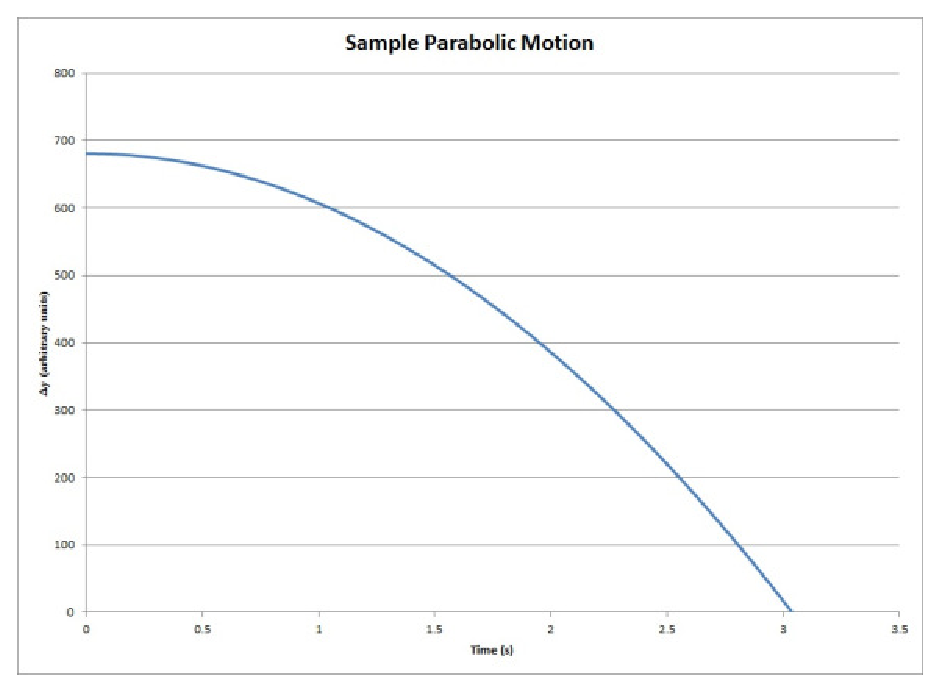
\includegraphics{parabolic_motion}
\caption[Parabolic Motion]{Here is parabolic motion as measured with science.}
\label{parabolic_motion}
\end{figure}
\lipsum
		
			
\begin{partChapter}
\chapter{Conclusion}

% the code below specifies where the figures are stored
\ifpdf
    \graphicspath{{colclusion/figures/PNG/}{colclusion/figures/PDF/}{colclusion/figures/}}
\else
    \graphicspath{{colclusion/figures/EPS/}{colclusion/figures/}}
\fi

% ----------------------------------------------------------------------
%: ----------------------- conclusion content ----------------------- 
% ----------------------------------------------------------------------

\section{Wrapping up\ldots}
I rest my case. \lipsum







\end{partChapter}
  

% --------------------------------------------------------------
%:                  BACK MATTER: appendices, refs,..
% --------------------------------------------------------------

%: ----------------------- Appendicies ------------------------
\begin{partChapter}

\begin{appendices}
\chapter{Some Appendix}
\lipsum
\section{first section}
\lipsum
\chapter{Another Appendix}
\lipsum
\end{appendices}

\end{partChapter}

% --------------------------------------------------------------
% backmatter mode set after appendix 
% any chapters beyond here have chapter number supressed
% --------------------------------------------------------------

\backmatter

%: ----------------------- glossary ------------------------

% Tie in external source file for definitions: /backmatter/glossary.tex
% Glossary entries can also be defined in the main text. See glossary.tex
% this file is called up by thesis.tex
% content in this file will be fed into the main document

% Glossary entries are defined with the command \nomenclature{1}{2}
% 1 = Entry name, e.g. abbreviation; 2 = Explanation
% You can place all explanations in this separate file or declare them in the middle of the text. Either way they will be collected in the glossary.

% required to print nomenclature name to page header
\markboth{\MakeUppercase{\nomname}}{\MakeUppercase{\nomname}}


% ----------------------- contents from here ------------------------

\nomenclature[Xe ]{11HUGS}{11 Mpc Halpha and Ultraviolet Galaxy Survey} 
\nomenclature[Zt ]{2MASS}{Two-Micron All Sky Sruvey}
\nomenclature[Am ]{M}{Mass of object}
\nomenclature[Gm ]{$\tau$}{Optical depth}
\nomenclature[Rs ]{$\ ^{*}$}{Conjugate}
\nomenclature[Ss ]{$\astrosun$}{relating to the sun (Sol)}
 

\clearpage
\begin{partChapter}
\begin{multicols}{2} % \begin{multicols}{#columns}[header text][space]
\begin{footnotesize} % scriptsize(7) < footnotesize(8) < small (9) < normal(10)

\printnomenclature[1.5cm] % [] = distance between entry and description
\label{nom} % target name for links to glossary

\end{footnotesize}
\end{multicols}
\end{partChapter}


% --------------------------------------------------------------
%: ----------------------- bibliography ------------------------
% --------------------------------------------------------------
% Various bibliography styles exist. Replace style as desired.

% For the following 4 bibliography styles:
% in-text refs: (1) (1; 2)
% ref list: alphabetical; author(s) in small caps; initials last name; page(s)
% PhDbiblio-case = title forced lower case
% PhDbiblio-bold = title as in bibtex but bold
% PhDbiblio-url = bold + www link if provided
% PhDbiblio-url2 = names small caps, title bold & hyperlinked, link to page 
% PhDbiblio-intext-twoauth= similar to PhDBiblio, with intext author citations 

% jmb = calls style file jmb
% in-text refs: author (year) without brackets
% ref list: alphabetical; author(s) in normal font; last name, initials; page(s)

%\bibliographystyle{plainnat} % calls style file plainnat.bst
% in-text refs: author (year) without brackets
% (this works with package natbib)
% --------------------------------------------------------------

\clearpage
\begin{partChapter}
%\begin{multicols}{1} % \begin{multicols}{ # columns}[ header text][ space]
\begin{footnotesize} % tiny(5) < scriptsize(7) < footnotesize(8) < small (9)

\bibliographystyle{Latex/Classes/PhDbiblio-url} % Title is link if provided
\renewcommand{\bibname}{References} % changes the header; default: Bibliography

\bibliography{./backmatter/references} % adjust this to fit your BibTex file

\end{footnotesize}
%\end{multicols}
\end{partChapter}



%: ----------------------- Index ------------------------
\clearpage
\begin{partChapter}
\printindex
\end{partChapter}


%: --------------------------------------------------------------
%:                     END OF DOCUMENT!!!
% --------------------------------------------------------------
\end{document}
